\documentclass[1p]{elsarticle_modified}
%\bibliographystyle{elsarticle-num}

%\usepackage[colorlinks]{hyperref}
%\usepackage{abbrmath_seonhwa} %\Abb, \Ascr, \Acal ,\Abf, \Afrak
\usepackage{amsfonts}
\usepackage{amssymb}
\usepackage{amsmath}
\usepackage{amsthm}
\usepackage{scalefnt}
\usepackage{amsbsy}
\usepackage{kotex}
\usepackage{caption}
\usepackage{subfig}
\usepackage{color}
\usepackage{graphicx}
\usepackage{xcolor} %% white, black, red, green, blue, cyan, magenta, yellow
\usepackage{float}
\usepackage{setspace}
\usepackage{hyperref}

\usepackage{tikz}
\usetikzlibrary{arrows}

\usepackage{multirow}
\usepackage{array} % fixed length table
\usepackage{hhline}

%%%%%%%%%%%%%%%%%%%%%
\makeatletter
\renewcommand*\env@matrix[1][\arraystretch]{%
	\edef\arraystretch{#1}%
	\hskip -\arraycolsep
	\let\@ifnextchar\new@ifnextchar
	\array{*\c@MaxMatrixCols c}}
\makeatother %https://tex.stackexchange.com/questions/14071/how-can-i-increase-the-line-spacing-in-a-matrix
%%%%%%%%%%%%%%%

\usepackage[normalem]{ulem}

\newcommand{\msout}[1]{\ifmmode\text{\sout{\ensuremath{#1}}}\else\sout{#1}\fi}
%SOURCE: \msout is \stkout macro in https://tex.stackexchange.com/questions/20609/strikeout-in-math-mode

\newcommand{\cancel}[1]{
	\ifmmode
	{\color{red}\msout{#1}}
	\else
	{\color{red}\sout{#1}}
	\fi
}

\newcommand{\add}[1]{
	{\color{blue}\uwave{#1}}
}

\newcommand{\replace}[2]{
	\ifmmode
	{\color{red}\msout{#1}}{\color{blue}\uwave{#2}}
	\else
	{\color{red}\sout{#1}}{\color{blue}\uwave{#2}}
	\fi
}

\newcommand{\Sol}{\mathcal{S}} %segment
\newcommand{\D}{D} %diagram
\newcommand{\A}{\mathcal{A}} %arc


%%%%%%%%%%%%%%%%%%%%%%%%%%%%%5 test

\def\sl{\operatorname{\textup{SL}}(2,\Cbb)}
\def\psl{\operatorname{\textup{PSL}}(2,\Cbb)}
\def\quan{\mkern 1mu \triangleright \mkern 1mu}

\theoremstyle{definition}
\newtheorem{thm}{Theorem}[section]
\newtheorem{prop}[thm]{Proposition}
\newtheorem{lem}[thm]{Lemma}
\newtheorem{ques}[thm]{Question}
\newtheorem{cor}[thm]{Corollary}
\newtheorem{defn}[thm]{Definition}
\newtheorem{exam}[thm]{Example}
\newtheorem{rmk}[thm]{Remark}
\newtheorem{alg}[thm]{Algorithm}

\newcommand{\I}{\sqrt{-1}}
\begin{document}

%\begin{frontmatter}
%
%\title{Boundary parabolic representations of knots up to 8 crossings}
%
%%% Group authors per affiliation:
%\author{Yunhi Cho} 
%\address{Department of Mathematics, University of Seoul, Seoul, Korea}
%\ead{yhcho@uos.ac.kr}
%
%
%\author{Seonhwa Kim} %\fnref{s_kim}}
%\address{Center for Geometry and Physics, Institute for Basic Science, Pohang, 37673, Korea}
%\ead{ryeona17@ibs.re.kr}
%
%\author{Hyuk Kim}
%\address{Department of Mathematical Sciences, Seoul National University, Seoul 08826, Korea}
%\ead{hyukkim@snu.ac.kr}
%
%\author{Seokbeom Yoon}
%\address{Department of Mathematical Sciences, Seoul National University, Seoul, 08826,  Korea}
%\ead{sbyoon15@snu.ac.kr}
%
%\begin{abstract}
%We find all boundary parabolic representation of knots up to 8 crossings.
%
%\end{abstract}
%\begin{keyword}
%    \MSC[2010] 57M25 
%\end{keyword}
%
%\end{frontmatter}

%\linenumbers
%\tableofcontents
%
\newcommand\colored[1]{\textcolor{white}{\rule[-0.35ex]{0.8em}{1.4ex}}\kern-0.8em\color{red} #1}%
%\newcommand\colored[1]{\textcolor{white}{ #1}\kern-2.17ex	\textcolor{white}{ #1}\kern-1.81ex	\textcolor{white}{ #1}\kern-2.15ex\color{red}#1	}

{\Large $\underline{12n_{0003}~(K12n_{0003})}$}

\setlength{\tabcolsep}{10pt}
\renewcommand{\arraystretch}{1.6}
\vspace{1cm}\begin{tabular}{m{100pt}>{\centering\arraybackslash}m{274pt}}
\multirow{5}{120pt}{
	\centering
	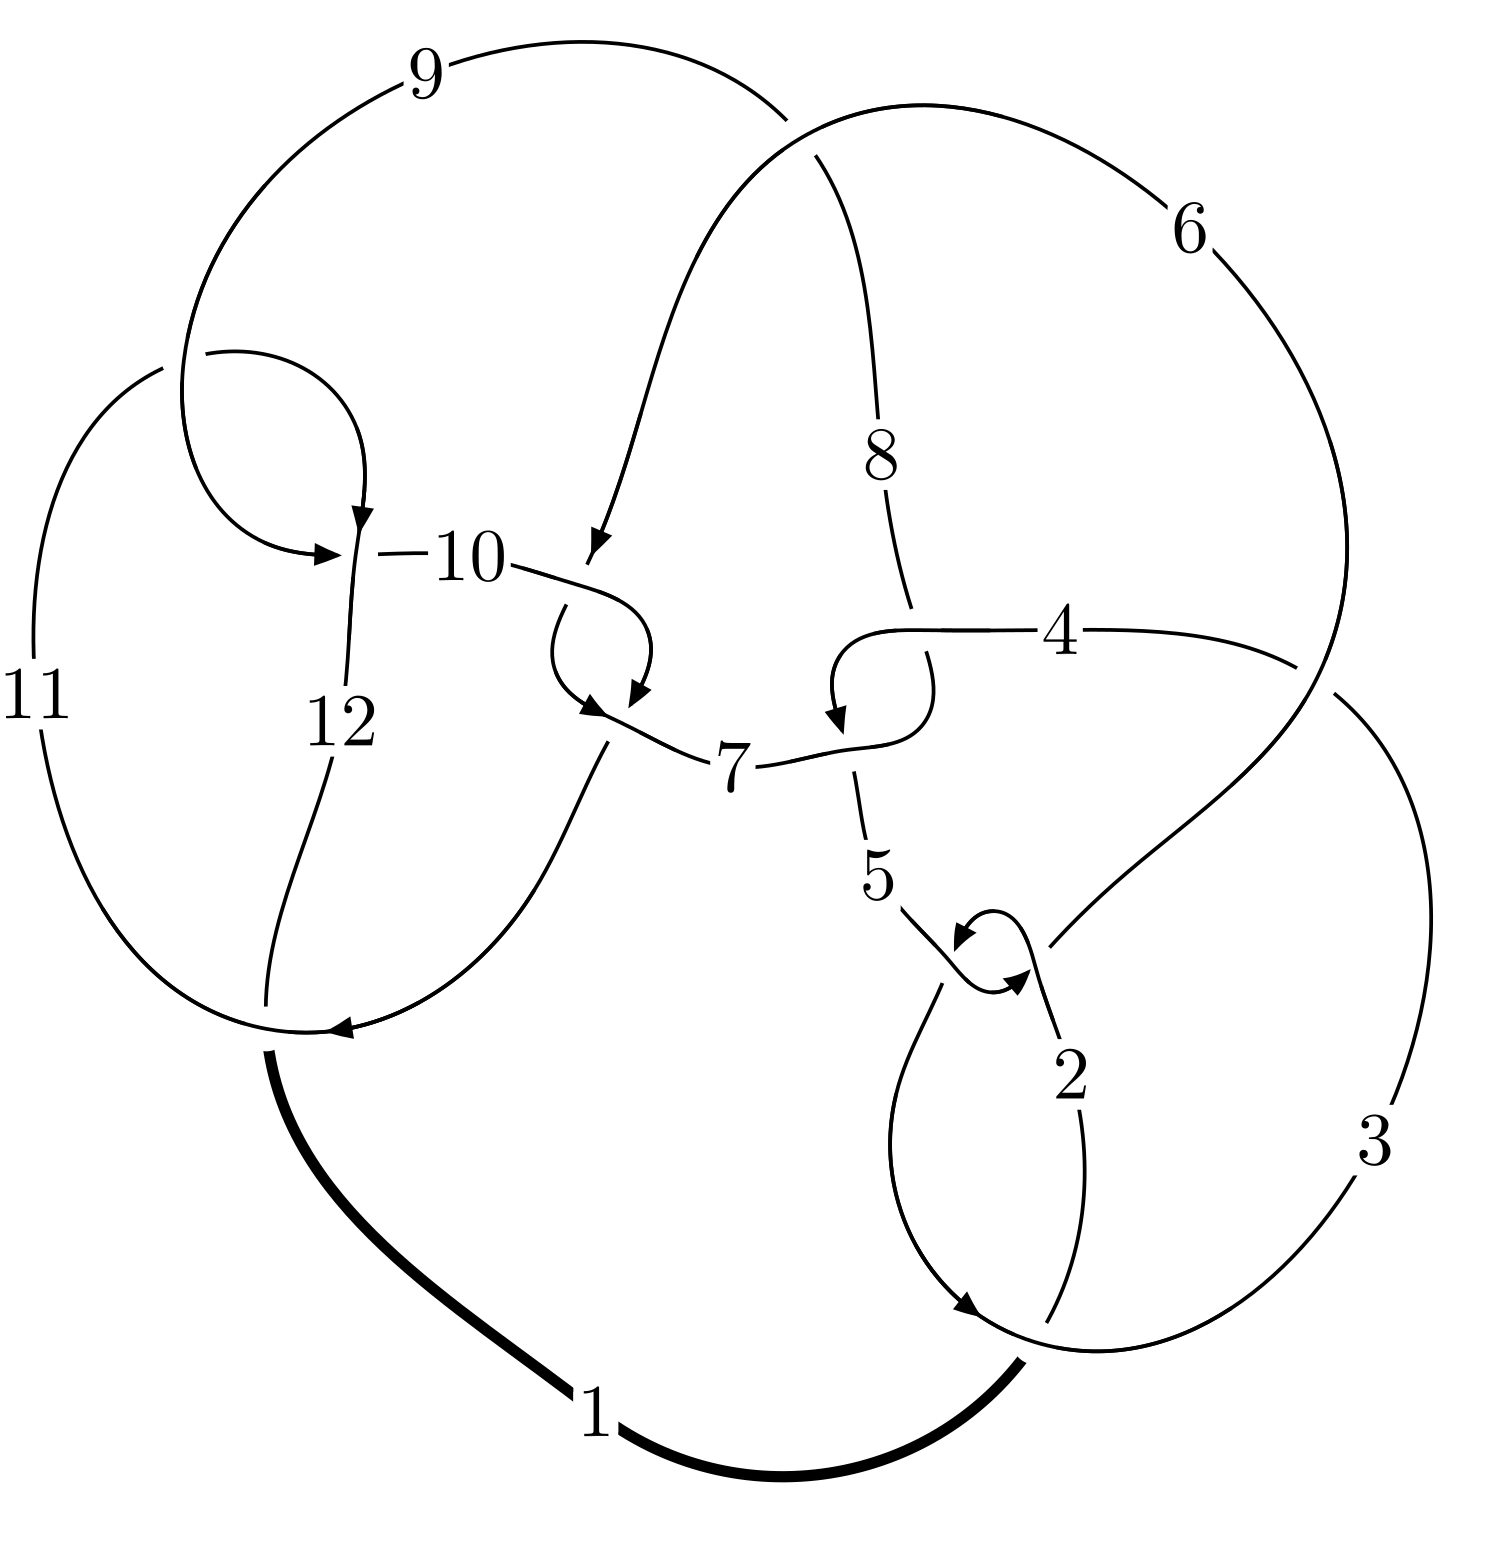
\includegraphics[width=112pt]{../../../GIT/diagram.site/Diagrams/png/2092_12n_0003.png}\\
\ \ \ A knot diagram\footnotemark}&
\allowdisplaybreaks
\textbf{Linearized knot diagam} \\
\cline{2-2}
 &
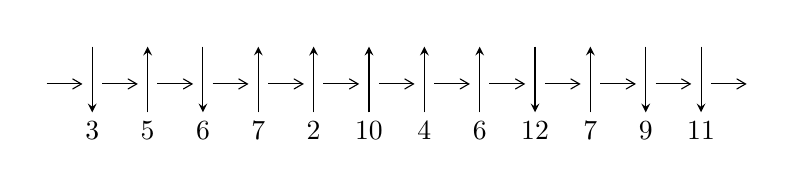
\begin{tikzpicture}[x=20pt, y=17pt]
	% nodes
	\node (C0) at (0, 0) {};
	\node (C1) at (1, 0) {};
	\node (C1U) at (1, +1) {};
	\node (C1D) at (1, -1) {3};

	\node (C2) at (2, 0) {};
	\node (C2U) at (2, +1) {};
	\node (C2D) at (2, -1) {5};

	\node (C3) at (3, 0) {};
	\node (C3U) at (3, +1) {};
	\node (C3D) at (3, -1) {6};

	\node (C4) at (4, 0) {};
	\node (C4U) at (4, +1) {};
	\node (C4D) at (4, -1) {7};

	\node (C5) at (5, 0) {};
	\node (C5U) at (5, +1) {};
	\node (C5D) at (5, -1) {2};

	\node (C6) at (6, 0) {};
	\node (C6U) at (6, +1) {};
	\node (C6D) at (6, -1) {10};

	\node (C7) at (7, 0) {};
	\node (C7U) at (7, +1) {};
	\node (C7D) at (7, -1) {4};

	\node (C8) at (8, 0) {};
	\node (C8U) at (8, +1) {};
	\node (C8D) at (8, -1) {6};

	\node (C9) at (9, 0) {};
	\node (C9U) at (9, +1) {};
	\node (C9D) at (9, -1) {12};

	\node (C10) at (10, 0) {};
	\node (C10U) at (10, +1) {};
	\node (C10D) at (10, -1) {7};

	\node (C11) at (11, 0) {};
	\node (C11U) at (11, +1) {};
	\node (C11D) at (11, -1) {9};

	\node (C12) at (12, 0) {};
	\node (C12U) at (12, +1) {};
	\node (C12D) at (12, -1) {11};
	\node (C13) at (13, 0) {};

	% arrows
	\draw[->,>={angle 60}]
	(C0) edge (C1) (C1) edge (C2) (C2) edge (C3) (C3) edge (C4) (C4) edge (C5) (C5) edge (C6) (C6) edge (C7) (C7) edge (C8) (C8) edge (C9) (C9) edge (C10) (C10) edge (C11) (C11) edge (C12) (C12) edge (C13) ;	\draw[->,>=stealth]
	(C1U) edge (C1D) (C2D) edge (C2U) (C3U) edge (C3D) (C4D) edge (C4U) (C5D) edge (C5U) (C6D) edge (C6U) (C7D) edge (C7U) (C8D) edge (C8U) (C9U) edge (C9D) (C10D) edge (C10U) (C11U) edge (C11D) (C12U) edge (C12D) ;
	\end{tikzpicture} \\
\hhline{~~} \\& 
\textbf{Solving Sequence} \\ \cline{2-2} 
 &
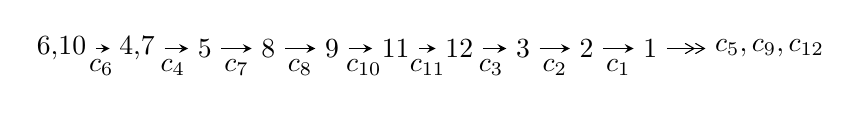
\begin{tikzpicture}[x=23pt, y=7pt]
	% node
	\node (A0) at (-1/8, 0) {6,10};
	\node (A1) at (17/16, 0) {4,7};
	\node (A2) at (17/8, 0) {5};
	\node (A3) at (25/8, 0) {8};
	\node (A4) at (33/8, 0) {9};
	\node (A5) at (41/8, 0) {11};
	\node (A6) at (49/8, 0) {12};
	\node (A7) at (57/8, 0) {3};
	\node (A8) at (65/8, 0) {2};
	\node (A9) at (73/8, 0) {1};
	\node (C1) at (1/2, -1) {$c_{6}$};
	\node (C2) at (13/8, -1) {$c_{4}$};
	\node (C3) at (21/8, -1) {$c_{7}$};
	\node (C4) at (29/8, -1) {$c_{8}$};
	\node (C5) at (37/8, -1) {$c_{10}$};
	\node (C6) at (45/8, -1) {$c_{11}$};
	\node (C7) at (53/8, -1) {$c_{3}$};
	\node (C8) at (61/8, -1) {$c_{2}$};
	\node (C9) at (69/8, -1) {$c_{1}$};
	\node (A10) at (11, 0) {$c_{5},c_{9},c_{12}$};

	% edge
	\draw[->,>=stealth]	
	(A0) edge (A1) (A1) edge (A2) (A2) edge (A3) (A3) edge (A4) (A4) edge (A5) (A5) edge (A6) (A6) edge (A7) (A7) edge (A8) (A8) edge (A9) ;
	\draw[->>,>={angle 60}]	
	(A9) edge (A10);
\end{tikzpicture} \\ 

\end{tabular} \\

\footnotetext{
The image of knot diagram is generated by the software ``\textbf{Draw programme}" developed by Andrew Bartholomew(\url{http://www.layer8.co.uk/maths/draw/index.htm\#Running-draw}), where we modified some parts for our purpose(\url{https://github.com/CATsTAILs/LinksPainter}).
}\phantom \\ \newline 
\centering \textbf{Ideals for irreducible components\footnotemark of $X_{\text{par}}$} 
 
\begin{align*}
I^u_{1}&=\langle 
-1.97857\times10^{48} u^{47}-8.37875\times10^{48} u^{46}+\cdots+1.28272\times10^{49} b+5.04932\times10^{48},\\
\phantom{I^u_{1}}&\phantom{= \langle  }-1.38689\times10^{49} u^{47}-4.12412\times10^{49} u^{46}+\cdots+1.28272\times10^{49} a-7.42829\times10^{49},\;u^{48}+3 u^{47}+\cdots+2 u+1\rangle \\
I^u_{2}&=\langle 
u^2 a+b,\;u^5 a+u^5-2 u^3 a-2 u^4+u^2 a- u^3+a^2+2 a u+3 u^2- a-2,\;u^6- u^5- u^4+2 u^3- u+1\rangle \\
\\
\end{align*}
\raggedright * 2 irreducible components of $\dim_{\mathbb{C}}=0$, with total 60 representations.\\
\footnotetext{All coefficients of polynomials are rational numbers. But the coefficients are sometimes approximated in decimal forms when there is not enough margin.}
\newpage
\renewcommand{\arraystretch}{1}
\centering \section*{I. $I^u_{1}= \langle -1.98\times10^{48} u^{47}-8.38\times10^{48} u^{46}+\cdots+1.28\times10^{49} b+5.05\times10^{48},\;-1.39\times10^{49} u^{47}-4.12\times10^{49} u^{46}+\cdots+1.28\times10^{49} a-7.43\times10^{49},\;u^{48}+3 u^{47}+\cdots+2 u+1 \rangle$}
\flushleft \textbf{(i) Arc colorings}\\
\begin{tabular}{m{7pt} m{180pt} m{7pt} m{180pt} }
\flushright $a_{6}=$&$\begin{pmatrix}1\\0\end{pmatrix}$ \\
\flushright $a_{10}=$&$\begin{pmatrix}0\\u\end{pmatrix}$ \\
\flushright $a_{4}=$&$\begin{pmatrix}1.08121 u^{47}+3.21513 u^{46}+\cdots+0.931628 u+5.79103\\0.154247 u^{47}+0.653200 u^{46}+\cdots-0.117415 u-0.393641\end{pmatrix}$ \\
\flushright $a_{7}=$&$\begin{pmatrix}1\\- u^2\end{pmatrix}$ \\
\flushright $a_{5}=$&$\begin{pmatrix}0.794887 u^{47}+2.62840 u^{46}+\cdots-0.210005 u+5.42589\\0.264517 u^{47}+0.943944 u^{46}+\cdots+0.140724 u-0.121410\end{pmatrix}$ \\
\flushright $a_{8}=$&$\begin{pmatrix}0.138808 u^{47}+0.0569367 u^{46}+\cdots+1.13835 u-1.23220\\0.0866426 u^{47}+0.143205 u^{46}+\cdots-0.0590538 u+0.156142\end{pmatrix}$ \\
\flushright $a_{9}=$&$\begin{pmatrix}0.225450 u^{47}+0.200142 u^{46}+\cdots+1.07929 u-1.07605\\0.0866426 u^{47}+0.143205 u^{46}+\cdots-0.0590538 u+0.156142\end{pmatrix}$ \\
\flushright $a_{11}=$&$\begin{pmatrix}u\\- u^3+u\end{pmatrix}$ \\
\flushright $a_{12}=$&$\begin{pmatrix}0.197793 u^{47}+0.746837 u^{46}+\cdots-0.411380 u+1.70840\\0.497798 u^{47}+1.23878 u^{46}+\cdots+1.17262 u+0.785808\end{pmatrix}$ \\
\flushright $a_{3}=$&$\begin{pmatrix}1.23546 u^{47}+3.86833 u^{46}+\cdots+0.814213 u+5.39739\\0.154247 u^{47}+0.653200 u^{46}+\cdots-0.117415 u-0.393641\end{pmatrix}$ \\
\flushright $a_{2}=$&$\begin{pmatrix}-1.23812 u^{47}-2.80513 u^{46}+\cdots-9.14389 u+0.0144920\\0.146826 u^{47}+0.655230 u^{46}+\cdots+0.00400667 u+0.694477\end{pmatrix}$ \\
\flushright $a_{1}=$&$\begin{pmatrix}0.138808 u^{47}+0.0569367 u^{46}+\cdots+1.13835 u-1.23220\\-0.270573 u^{47}-0.659768 u^{46}+\cdots-0.521111 u-0.515628\end{pmatrix}$\\&\end{tabular}
\flushleft \textbf{(ii) Obstruction class $= -1$}\\~\\
\flushleft \textbf{(iii) Cusp Shapes $= 7.13383 u^{47}+19.7832 u^{46}+\cdots+16.2053 u+20.7902$}\\~\\
\newpage\renewcommand{\arraystretch}{1}
\flushleft \textbf{(iv) u-Polynomials at the component}\newline \\
\begin{tabular}{m{50pt}|m{274pt}}
Crossings & \hspace{64pt}u-Polynomials at each crossing \\
\hline $$\begin{aligned}c_{1}\end{aligned}$$&$\begin{aligned}
&u^{48}+31 u^{47}+\cdots+24 u+1
\end{aligned}$\\
\hline $$\begin{aligned}c_{2},c_{5}\end{aligned}$$&$\begin{aligned}
&u^{48}+7 u^{47}+\cdots+12 u+1
\end{aligned}$\\
\hline $$\begin{aligned}c_{3}\end{aligned}$$&$\begin{aligned}
&u^{48}-7 u^{47}+\cdots+12 u^2+1
\end{aligned}$\\
\hline $$\begin{aligned}c_{4},c_{7}\end{aligned}$$&$\begin{aligned}
&u^{48}+3 u^{47}+\cdots-8192 u+4096
\end{aligned}$\\
\hline $$\begin{aligned}c_{6},c_{10}\end{aligned}$$&$\begin{aligned}
&u^{48}-3 u^{47}+\cdots-2 u+1
\end{aligned}$\\
\hline $$\begin{aligned}c_{8}\end{aligned}$$&$\begin{aligned}
&u^{48}+9 u^{47}+\cdots-23626848 u+3579401
\end{aligned}$\\
\hline $$\begin{aligned}c_{9},c_{11}\end{aligned}$$&$\begin{aligned}
&u^{48}-3 u^{47}+\cdots-8 u+1
\end{aligned}$\\
\hline $$\begin{aligned}c_{12}\end{aligned}$$&$\begin{aligned}
&u^{48}+29 u^{47}+\cdots+8 u+1
\end{aligned}$\\
\hline
\end{tabular}\\~\\
\newpage\renewcommand{\arraystretch}{1}
\flushleft \textbf{(v) Riley Polynomials at the component}\newline \\
\begin{tabular}{m{50pt}|m{274pt}}
Crossings & \hspace{64pt}Riley Polynomials at each crossing \\
\hline $$\begin{aligned}c_{1}\end{aligned}$$&$\begin{aligned}
&y^{48}-21 y^{47}+\cdots+2824 y+1
\end{aligned}$\\
\hline $$\begin{aligned}c_{2},c_{5}\end{aligned}$$&$\begin{aligned}
&y^{48}+31 y^{47}+\cdots+24 y+1
\end{aligned}$\\
\hline $$\begin{aligned}c_{3}\end{aligned}$$&$\begin{aligned}
&y^{48}-73 y^{47}+\cdots+24 y+1
\end{aligned}$\\
\hline $$\begin{aligned}c_{4},c_{7}\end{aligned}$$&$\begin{aligned}
&y^{48}+65 y^{47}+\cdots+184549376 y+16777216
\end{aligned}$\\
\hline $$\begin{aligned}c_{6},c_{10}\end{aligned}$$&$\begin{aligned}
&y^{48}-9 y^{47}+\cdots-8 y+1
\end{aligned}$\\
\hline $$\begin{aligned}c_{8}\end{aligned}$$&$\begin{aligned}
&y^{48}+83 y^{47}+\cdots+697935129971156 y+12812111518801
\end{aligned}$\\
\hline $$\begin{aligned}c_{9},c_{11}\end{aligned}$$&$\begin{aligned}
&y^{48}-29 y^{47}+\cdots-8 y+1
\end{aligned}$\\
\hline $$\begin{aligned}c_{12}\end{aligned}$$&$\begin{aligned}
&y^{48}-17 y^{47}+\cdots+200 y+1
\end{aligned}$\\
\hline
\end{tabular}\\~\\
\newpage\flushleft \textbf{(vi) Complex Volumes and Cusp Shapes}
$$\begin{array}{c|c|c}  
\text{Solutions to }I^u_{1}& \I (\text{vol} + \sqrt{-1}CS) & \text{Cusp shape}\\
 \hline 
\begin{aligned}
u &= \phantom{-}0.888432 + 0.471966 I \\
a &= -0.334610 - 1.300970 I \\
b &= -0.050019 + 0.219961 I\end{aligned}
 & -4.63723 - 0.72636 I & -3.19086 - 0.34526 I \\ \hline\begin{aligned}
u &= \phantom{-}0.888432 - 0.471966 I \\
a &= -0.334610 + 1.300970 I \\
b &= -0.050019 - 0.219961 I\end{aligned}
 & -4.63723 + 0.72636 I & -3.19086 + 0.34526 I \\ \hline\begin{aligned}
u &= \phantom{-}0.636986 + 0.733622 I \\
a &= \phantom{-}0.279122 + 0.849564 I \\
b &= -0.813791 - 0.933020 I\end{aligned}
 & -5.67745 + 5.32167 I & -4.21900 - 6.97135 I \\ \hline\begin{aligned}
u &= \phantom{-}0.636986 - 0.733622 I \\
a &= \phantom{-}0.279122 - 0.849564 I \\
b &= -0.813791 + 0.933020 I\end{aligned}
 & -5.67745 - 5.32167 I & -4.21900 + 6.97135 I \\ \hline\begin{aligned}
u &= -1.035480 + 0.144515 I \\
a &= \phantom{-}0.398707 + 0.045146 I \\
b &= -0.005777 - 0.451241 I\end{aligned}
 & \phantom{-}1.83509 - 0.11544 I & \phantom{-}4.43775 + 1.73282 I \\ \hline\begin{aligned}
u &= -1.035480 - 0.144515 I \\
a &= \phantom{-}0.398707 - 0.045146 I \\
b &= -0.005777 + 0.451241 I\end{aligned}
 & \phantom{-}1.83509 + 0.11544 I & \phantom{-}4.43775 - 1.73282 I \\ \hline\begin{aligned}
u &= \phantom{-}0.468363 + 0.992714 I \\
a &= -0.028122 + 0.951893 I \\
b &= \phantom{-}0.197854 - 0.122368 I\end{aligned}
 & -3.89164 - 1.83510 I & -3.88038 + 1.67120 I \\ \hline\begin{aligned}
u &= \phantom{-}0.468363 - 0.992714 I \\
a &= -0.028122 - 0.951893 I \\
b &= \phantom{-}0.197854 + 0.122368 I\end{aligned}
 & -3.89164 + 1.83510 I & -3.88038 - 1.67120 I \\ \hline\begin{aligned}
u &= -0.438971 + 0.749800 I \\
a &= -0.150656 - 0.909768 I \\
b &= -0.434634 + 0.073940 I\end{aligned}
 & -1.87656 - 2.26693 I & -0.23419 + 4.23054 I \\ \hline\begin{aligned}
u &= -0.438971 - 0.749800 I \\
a &= -0.150656 + 0.909768 I \\
b &= -0.434634 - 0.073940 I\end{aligned}
 & -1.87656 + 2.26693 I & -0.23419 - 4.23054 I\\
 \hline 
 \end{array}$$\newpage$$\begin{array}{c|c|c}  
\text{Solutions to }I^u_{1}& \I (\text{vol} + \sqrt{-1}CS) & \text{Cusp shape}\\
 \hline 
\begin{aligned}
u &= \phantom{-}1.055170 + 0.454319 I \\
a &= \phantom{-}0.350993 - 0.350907 I \\
b &= -0.229165 + 0.586958 I\end{aligned}
 & \phantom{-}0.47415 + 4.77230 I & \phantom{-}2.90925 - 7.59230 I \\ \hline\begin{aligned}
u &= \phantom{-}1.055170 - 0.454319 I \\
a &= \phantom{-}0.350993 + 0.350907 I \\
b &= -0.229165 - 0.586958 I\end{aligned}
 & \phantom{-}0.47415 - 4.77230 I & \phantom{-}2.90925 + 7.59230 I \\ \hline\begin{aligned}
u &= -1.157600 + 0.418766 I \\
a &= -0.250131 + 0.368235 I \\
b &= \phantom{-}0.366611 + 0.145765 I\end{aligned}
 & \phantom{-}0.69730 - 2.30425 I & \phantom{-0.000000 } 0 \\ \hline\begin{aligned}
u &= -1.157600 - 0.418766 I \\
a &= -0.250131 - 0.368235 I \\
b &= \phantom{-}0.366611 - 0.145765 I\end{aligned}
 & \phantom{-}0.69730 + 2.30425 I & \phantom{-0.000000 } 0 \\ \hline\begin{aligned}
u &= -0.617941 + 0.399224 I \\
a &= \phantom{-}0.060615 + 0.914870 I \\
b &= -1.57348 - 1.15912 I\end{aligned}
 & -1.23836 - 4.95401 I & \phantom{-}0.95024 + 9.76424 I \\ \hline\begin{aligned}
u &= -0.617941 - 0.399224 I \\
a &= \phantom{-}0.060615 - 0.914870 I \\
b &= -1.57348 + 1.15912 I\end{aligned}
 & -1.23836 + 4.95401 I & \phantom{-}0.95024 - 9.76424 I \\ \hline\begin{aligned}
u &= -0.690433 + 0.022710 I \\
a &= \phantom{-}0.340123 + 0.236436 I \\
b &= \phantom{-}0.710419 - 0.336425 I\end{aligned}
 & \phantom{-}1.274320 - 0.061861 I & \phantom{-}8.91275 - 0.63325 I \\ \hline\begin{aligned}
u &= -0.690433 - 0.022710 I \\
a &= \phantom{-}0.340123 - 0.236436 I \\
b &= \phantom{-}0.710419 + 0.336425 I\end{aligned}
 & \phantom{-}1.274320 + 0.061861 I & \phantom{-}8.91275 + 0.63325 I \\ \hline\begin{aligned}
u &= \phantom{-}0.952290 + 0.917135 I \\
a &= \phantom{-}0.86871 - 1.24612 I \\
b &= -2.02867 + 0.31602 I\end{aligned}
 & -5.72498 + 3.38721 I & \phantom{-0.000000 } 0 \\ \hline\begin{aligned}
u &= \phantom{-}0.952290 - 0.917135 I \\
a &= \phantom{-}0.86871 + 1.24612 I \\
b &= -2.02867 - 0.31602 I\end{aligned}
 & -5.72498 - 3.38721 I & \phantom{-0.000000 } 0\\
 \hline 
 \end{array}$$\newpage$$\begin{array}{c|c|c}  
\text{Solutions to }I^u_{1}& \I (\text{vol} + \sqrt{-1}CS) & \text{Cusp shape}\\
 \hline 
\begin{aligned}
u &= \phantom{-}0.663259 + 0.139973 I \\
a &= \phantom{-}0.219248 - 1.384360 I \\
b &= \phantom{-}0.12321 + 1.65156 I\end{aligned}
 & \phantom{-}0.85103 + 2.84744 I & \phantom{-}6.69474 - 7.55737 I \\ \hline\begin{aligned}
u &= \phantom{-}0.663259 - 0.139973 I \\
a &= \phantom{-}0.219248 + 1.384360 I \\
b &= \phantom{-}0.12321 - 1.65156 I\end{aligned}
 & \phantom{-}0.85103 - 2.84744 I & \phantom{-}6.69474 + 7.55737 I \\ \hline\begin{aligned}
u &= -0.864759 + 1.001780 I \\
a &= -0.70764 - 1.33859 I \\
b &= \phantom{-}2.09539 + 0.70588 I\end{aligned}
 & -14.6682 - 3.0850 I & \phantom{-0.000000 } 0 \\ \hline\begin{aligned}
u &= -0.864759 - 1.001780 I \\
a &= -0.70764 + 1.33859 I \\
b &= \phantom{-}2.09539 - 0.70588 I\end{aligned}
 & -14.6682 + 3.0850 I & \phantom{-0.000000 } 0 \\ \hline\begin{aligned}
u &= -0.934317 + 0.943776 I \\
a &= \phantom{-}1.07851 + 1.19683 I \\
b &= -2.15162 + 0.09289 I\end{aligned}
 & -9.73534 + 1.58904 I & \phantom{-0.000000 } 0 \\ \hline\begin{aligned}
u &= -0.934317 - 0.943776 I \\
a &= \phantom{-}1.07851 - 1.19683 I \\
b &= -2.15162 - 0.09289 I\end{aligned}
 & -9.73534 - 1.58904 I & \phantom{-0.000000 } 0 \\ \hline\begin{aligned}
u &= \phantom{-}0.325135 + 0.583617 I \\
a &= \phantom{-}1.010560 - 0.435996 I \\
b &= -0.100686 - 0.124770 I\end{aligned}
 & -1.73157 - 0.74220 I & -3.53436 + 1.20207 I \\ \hline\begin{aligned}
u &= \phantom{-}0.325135 - 0.583617 I \\
a &= \phantom{-}1.010560 + 0.435996 I \\
b &= -0.100686 + 0.124770 I\end{aligned}
 & -1.73157 + 0.74220 I & -3.53436 - 1.20207 I \\ \hline\begin{aligned}
u &= \phantom{-}1.213470 + 0.584928 I \\
a &= -0.504959 - 0.128402 I \\
b &= \phantom{-}0.658444 - 0.124156 I\end{aligned}
 & -1.32166 + 7.73642 I & \phantom{-0.000000 } 0 \\ \hline\begin{aligned}
u &= \phantom{-}1.213470 - 0.584928 I \\
a &= -0.504959 + 0.128402 I \\
b &= \phantom{-}0.658444 + 0.124156 I\end{aligned}
 & -1.32166 - 7.73642 I & \phantom{-0.000000 } 0\\
 \hline 
 \end{array}$$\newpage$$\begin{array}{c|c|c}  
\text{Solutions to }I^u_{1}& \I (\text{vol} + \sqrt{-1}CS) & \text{Cusp shape}\\
 \hline 
\begin{aligned}
u &= -0.978343 + 0.926207 I \\
a &= \phantom{-}0.80633 + 1.44174 I \\
b &= -2.29946 - 0.61084 I\end{aligned}
 & -9.59881 - 8.46951 I & \phantom{-0.000000 } 0 \\ \hline\begin{aligned}
u &= -0.978343 - 0.926207 I \\
a &= \phantom{-}0.80633 - 1.44174 I \\
b &= -2.29946 + 0.61084 I\end{aligned}
 & -9.59881 + 8.46951 I & \phantom{-0.000000 } 0 \\ \hline\begin{aligned}
u &= \phantom{-}0.866755 + 1.048470 I \\
a &= -0.729094 + 1.119430 I \\
b &= \phantom{-}1.93255 - 0.26341 I\end{aligned}
 & -10.22760 - 1.78431 I & \phantom{-0.000000 } 0 \\ \hline\begin{aligned}
u &= \phantom{-}0.866755 - 1.048470 I \\
a &= -0.729094 - 1.119430 I \\
b &= \phantom{-}1.93255 + 0.26341 I\end{aligned}
 & -10.22760 + 1.78431 I & \phantom{-0.000000 } 0 \\ \hline\begin{aligned}
u &= -1.051530 + 0.891321 I \\
a &= -1.31485 - 1.07651 I \\
b &= \phantom{-}2.10442 - 0.11160 I\end{aligned}
 & -14.0441 - 3.8628 I & \phantom{-0.000000 } 0 \\ \hline\begin{aligned}
u &= -1.051530 - 0.891321 I \\
a &= -1.31485 + 1.07651 I \\
b &= \phantom{-}2.10442 + 0.11160 I\end{aligned}
 & -14.0441 + 3.8628 I & \phantom{-0.000000 } 0 \\ \hline\begin{aligned}
u &= -0.905222 + 1.060420 I \\
a &= -0.888396 - 1.029930 I \\
b &= \phantom{-}2.14464 - 0.04344 I\end{aligned}
 & -13.8372 + 7.1481 I & \phantom{-0.000000 } 0 \\ \hline\begin{aligned}
u &= -0.905222 - 1.060420 I \\
a &= -0.888396 + 1.029930 I \\
b &= \phantom{-}2.14464 + 0.04344 I\end{aligned}
 & -13.8372 - 7.1481 I & \phantom{-0.000000 } 0 \\ \hline\begin{aligned}
u &= \phantom{-}1.07786 + 0.91788 I \\
a &= -1.00742 + 1.16837 I \\
b &= \phantom{-}2.09175 - 0.23831 I\end{aligned}
 & -9.52196 + 8.95742 I & \phantom{-0.000000 } 0 \\ \hline\begin{aligned}
u &= \phantom{-}1.07786 - 0.91788 I \\
a &= -1.00742 - 1.16837 I \\
b &= \phantom{-}2.09175 + 0.23831 I\end{aligned}
 & -9.52196 - 8.95742 I & \phantom{-0.000000 } 0\\
 \hline 
 \end{array}$$\newpage$$\begin{array}{c|c|c}  
\text{Solutions to }I^u_{1}& \I (\text{vol} + \sqrt{-1}CS) & \text{Cusp shape}\\
 \hline 
\begin{aligned}
u &= -1.06846 + 0.94471 I \\
a &= -0.91395 - 1.39925 I \\
b &= \phantom{-}2.30191 + 0.42350 I\end{aligned}
 & -13.2732 - 14.4519 I & \phantom{-0.000000 } 0 \\ \hline\begin{aligned}
u &= -1.06846 - 0.94471 I \\
a &= -0.91395 + 1.39925 I \\
b &= \phantom{-}2.30191 - 0.42350 I\end{aligned}
 & -13.2732 + 14.4519 I & \phantom{-0.000000 } 0 \\ \hline\begin{aligned}
u &= \phantom{-}0.518541 + 0.209657 I \\
a &= -0.15012 - 2.09948 I \\
b &= -0.571793 + 1.215850 I\end{aligned}
 & \phantom{-}0.60718 + 2.45344 I & \phantom{-}2.01156 - 2.44263 I \\ \hline\begin{aligned}
u &= \phantom{-}0.518541 - 0.209657 I \\
a &= -0.15012 + 2.09948 I \\
b &= -0.571793 - 1.215850 I\end{aligned}
 & \phantom{-}0.60718 - 2.45344 I & \phantom{-}2.01156 + 2.44263 I \\ \hline\begin{aligned}
u &= -0.097000 + 0.527699 I \\
a &= -0.97037 - 3.44326 I \\
b &= -0.320461 - 0.724196 I\end{aligned}
 & -1.36020 - 1.48509 I & -1.96785 + 10.33925 I \\ \hline\begin{aligned}
u &= -0.097000 - 0.527699 I \\
a &= -0.97037 + 3.44326 I \\
b &= -0.320461 + 0.724196 I\end{aligned}
 & -1.36020 + 1.48509 I & -1.96785 - 10.33925 I \\ \hline\begin{aligned}
u &= -0.326195 + 0.340981 I \\
a &= \phantom{-}4.53740 + 4.91757 I \\
b &= -0.647629 + 0.837735 I\end{aligned}
 & -1.80837 + 2.42279 I & \phantom{-}4.5070 + 19.1208 I \\ \hline\begin{aligned}
u &= -0.326195 - 0.340981 I \\
a &= \phantom{-}4.53740 - 4.91757 I \\
b &= -0.647629 - 0.837735 I\end{aligned}
 & -1.80837 - 2.42279 I & \phantom{-}4.5070 - 19.1208 I\\
 \hline 
 \end{array}$$\newpage\newpage\renewcommand{\arraystretch}{1}
\centering \section*{II. $I^u_{2}= \langle u^2 a+b,\;u^5 a+u^5+\cdots- a-2,\;u^6- u^5- u^4+2 u^3- u+1 \rangle$}
\flushleft \textbf{(i) Arc colorings}\\
\begin{tabular}{m{7pt} m{180pt} m{7pt} m{180pt} }
\flushright $a_{6}=$&$\begin{pmatrix}1\\0\end{pmatrix}$ \\
\flushright $a_{10}=$&$\begin{pmatrix}0\\u\end{pmatrix}$ \\
\flushright $a_{4}=$&$\begin{pmatrix}a\\- u^2 a\end{pmatrix}$ \\
\flushright $a_{7}=$&$\begin{pmatrix}1\\- u^2\end{pmatrix}$ \\
\flushright $a_{5}=$&$\begin{pmatrix}a\\- u^2 a\end{pmatrix}$ \\
\flushright $a_{8}=$&$\begin{pmatrix}1\\- u^2\end{pmatrix}$ \\
\flushright $a_{9}=$&$\begin{pmatrix}- u^2+1\\- u^2\end{pmatrix}$ \\
\flushright $a_{11}=$&$\begin{pmatrix}u\\- u^3+u\end{pmatrix}$ \\
\flushright $a_{12}=$&$\begin{pmatrix}- u^4+u^2-1\\u^5- u^4-2 u^3+u^2+u-1\end{pmatrix}$ \\
\flushright $a_{3}=$&$\begin{pmatrix}- u^2 a+a\\- u^2 a\end{pmatrix}$ \\
\flushright $a_{2}=$&$\begin{pmatrix}u^5- u^2 a-2 u^3+u^2+a+2 u-1\\- u^2 a+1\end{pmatrix}$ \\
\flushright $a_{1}=$&$\begin{pmatrix}-1\\0\end{pmatrix}$\\&\end{tabular}
\flushleft \textbf{(ii) Obstruction class $= 1$}\\~\\
\flushleft \textbf{(iii) Cusp Shapes $= 2 u^5 a+u^4 a+u^5-4 u^3 a-6 u^4+5 u^2 a- u^3+3 a u+7 u^2-2 a-4 u-4$}\\~\\
\newpage\renewcommand{\arraystretch}{1}
\flushleft \textbf{(iv) u-Polynomials at the component}\newline \\
\begin{tabular}{m{50pt}|m{274pt}}
Crossings & \hspace{64pt}u-Polynomials at each crossing \\
\hline $$\begin{aligned}c_{1},c_{3},c_{5}\end{aligned}$$&$\begin{aligned}
&(u^2- u+1)^6
\end{aligned}$\\
\hline $$\begin{aligned}c_{2}\end{aligned}$$&$\begin{aligned}
&(u^2+u+1)^6
\end{aligned}$\\
\hline $$\begin{aligned}c_{4},c_{7}\end{aligned}$$&$\begin{aligned}
&u^{12}
\end{aligned}$\\
\hline $$\begin{aligned}c_{6},c_{11}\end{aligned}$$&$\begin{aligned}
&(u^6- u^5- u^4+2 u^3- u+1)^2
\end{aligned}$\\
\hline $$\begin{aligned}c_{8}\end{aligned}$$&$\begin{aligned}
&(u^6-3 u^5+5 u^4-4 u^3+2 u^2- u+1)^2
\end{aligned}$\\
\hline $$\begin{aligned}c_{9},c_{10}\end{aligned}$$&$\begin{aligned}
&(u^6+u^5- u^4-2 u^3+u+1)^2
\end{aligned}$\\
\hline $$\begin{aligned}c_{12}\end{aligned}$$&$\begin{aligned}
&(u^6+3 u^5+5 u^4+4 u^3+2 u^2+u+1)^2
\end{aligned}$\\
\hline
\end{tabular}\\~\\
\newpage\renewcommand{\arraystretch}{1}
\flushleft \textbf{(v) Riley Polynomials at the component}\newline \\
\begin{tabular}{m{50pt}|m{274pt}}
Crossings & \hspace{64pt}Riley Polynomials at each crossing \\
\hline $$\begin{aligned}c_{1},c_{2},c_{3}\\c_{5}\end{aligned}$$&$\begin{aligned}
&(y^2+y+1)^6
\end{aligned}$\\
\hline $$\begin{aligned}c_{4},c_{7}\end{aligned}$$&$\begin{aligned}
&y^{12}
\end{aligned}$\\
\hline $$\begin{aligned}c_{6},c_{9},c_{10}\\c_{11}\end{aligned}$$&$\begin{aligned}
&(y^6-3 y^5+5 y^4-4 y^3+2 y^2- y+1)^2
\end{aligned}$\\
\hline $$\begin{aligned}c_{8},c_{12}\end{aligned}$$&$\begin{aligned}
&(y^6+y^5+5 y^4+6 y^2+3 y+1)^2
\end{aligned}$\\
\hline
\end{tabular}\\~\\
\newpage\flushleft \textbf{(vi) Complex Volumes and Cusp Shapes}
$$\begin{array}{c|c|c}  
\text{Solutions to }I^u_{2}& \I (\text{vol} + \sqrt{-1}CS) & \text{Cusp shape}\\
 \hline 
\begin{aligned}
u &= -1.002190 + 0.295542 I \\
a &= \phantom{-}0.815127 - 0.417821 I \\
b &= -0.500000 + 0.866025 I\end{aligned}
 & \phantom{-}1.89061 + 1.10558 I & \phantom{-}4.53097 - 2.95636 I \\ \hline\begin{aligned}
u &= -1.002190 + 0.295542 I \\
a &= -0.045720 + 0.914831 I \\
b &= -0.500000 - 0.866025 I\end{aligned}
 & \phantom{-}1.89061 - 2.95419 I & \phantom{-}7.73749 + 4.22314 I \\ \hline\begin{aligned}
u &= -1.002190 - 0.295542 I \\
a &= \phantom{-}0.815127 + 0.417821 I \\
b &= -0.500000 - 0.866025 I\end{aligned}
 & \phantom{-}1.89061 - 1.10558 I & \phantom{-}4.53097 + 2.95636 I \\ \hline\begin{aligned}
u &= -1.002190 - 0.295542 I \\
a &= -0.045720 - 0.914831 I \\
b &= -0.500000 + 0.866025 I\end{aligned}
 & \phantom{-}1.89061 + 2.95419 I & \phantom{-}7.73749 - 4.22314 I \\ \hline\begin{aligned}
u &= \phantom{-}0.428243 + 0.664531 I \\
a &= \phantom{-}0.93136 - 1.30101 I \\
b &= -0.500000 - 0.866025 I\end{aligned}
 & -1.89061 - 2.95419 I & -0.76561 + 6.31197 I \\ \hline\begin{aligned}
u &= \phantom{-}0.428243 + 0.664531 I \\
a &= -1.59239 - 0.15607 I \\
b &= -0.500000 + 0.866025 I\end{aligned}
 & -1.89061 + 1.10558 I & -4.61123 - 3.09109 I \\ \hline\begin{aligned}
u &= \phantom{-}0.428243 - 0.664531 I \\
a &= \phantom{-}0.93136 + 1.30101 I \\
b &= -0.500000 + 0.866025 I\end{aligned}
 & -1.89061 + 2.95419 I & -0.76561 - 6.31197 I \\ \hline\begin{aligned}
u &= \phantom{-}0.428243 - 0.664531 I \\
a &= -1.59239 + 0.15607 I \\
b &= -0.500000 - 0.866025 I\end{aligned}
 & -1.89061 - 1.10558 I & -4.61123 + 3.09109 I \\ \hline\begin{aligned}
u &= \phantom{-}1.073950 + 0.558752 I \\
a &= \phantom{-}0.679704 + 0.059778 I \\
b &= -0.500000 - 0.866025 I\end{aligned}
 & \phantom{-0.000000 -}3.66314 I & -0.57335 - 1.75283 I \\ \hline\begin{aligned}
u &= \phantom{-}1.073950 + 0.558752 I \\
a &= -0.288082 - 0.618530 I \\
b &= -0.500000 + 0.866025 I\end{aligned}
 & \phantom{-0.000000 -}7.72290 I & \phantom{-}3.68173 - 7.68692 I\\
 \hline 
 \end{array}$$\newpage$$\begin{array}{c|c|c}  
\text{Solutions to }I^u_{2}& \I (\text{vol} + \sqrt{-1}CS) & \text{Cusp shape}\\
 \hline 
\begin{aligned}
u &= \phantom{-}1.073950 - 0.558752 I \\
a &= \phantom{-}0.679704 - 0.059778 I \\
b &= -0.500000 + 0.866025 I\end{aligned}
 & \phantom{-0.000000 } -3.66314 I & -0.57335 + 1.75283 I \\ \hline\begin{aligned}
u &= \phantom{-}1.073950 - 0.558752 I \\
a &= -0.288082 + 0.618530 I \\
b &= -0.500000 - 0.866025 I\end{aligned}
 & \phantom{-0.000000 } -7.72290 I & \phantom{-}3.68173 + 7.68692 I\\
 \hline 
 \end{array}$$\newpage
\newpage\renewcommand{\arraystretch}{1}
\centering \section*{ III. u-Polynomials}
\begin{tabular}{m{50pt}|m{274pt}}
Crossings & \hspace{64pt}u-Polynomials at each crossing \\
\hline $$\begin{aligned}c_{1}\end{aligned}$$&$\begin{aligned}
&((u^2- u+1)^6)(u^{48}+31 u^{47}+\cdots+24 u+1)
\end{aligned}$\\
\hline $$\begin{aligned}c_{2}\end{aligned}$$&$\begin{aligned}
&((u^2+u+1)^6)(u^{48}+7 u^{47}+\cdots+12 u+1)
\end{aligned}$\\
\hline $$\begin{aligned}c_{3}\end{aligned}$$&$\begin{aligned}
&((u^2- u+1)^6)(u^{48}-7 u^{47}+\cdots+12 u^2+1)
\end{aligned}$\\
\hline $$\begin{aligned}c_{4},c_{7}\end{aligned}$$&$\begin{aligned}
&u^{12}(u^{48}+3 u^{47}+\cdots-8192 u+4096)
\end{aligned}$\\
\hline $$\begin{aligned}c_{5}\end{aligned}$$&$\begin{aligned}
&((u^2- u+1)^6)(u^{48}+7 u^{47}+\cdots+12 u+1)
\end{aligned}$\\
\hline $$\begin{aligned}c_{6}\end{aligned}$$&$\begin{aligned}
&((u^6- u^5- u^4+2 u^3- u+1)^2)(u^{48}-3 u^{47}+\cdots-2 u+1)
\end{aligned}$\\
\hline $$\begin{aligned}c_{8}\end{aligned}$$&$\begin{aligned}
&(u^6-3 u^5+5 u^4-4 u^3+2 u^2- u+1)^2\\
&\cdot(u^{48}+9 u^{47}+\cdots-23626848 u+3579401)
\end{aligned}$\\
\hline $$\begin{aligned}c_{9}\end{aligned}$$&$\begin{aligned}
&((u^6+u^5- u^4-2 u^3+u+1)^2)(u^{48}-3 u^{47}+\cdots-8 u+1)
\end{aligned}$\\
\hline $$\begin{aligned}c_{10}\end{aligned}$$&$\begin{aligned}
&((u^6+u^5- u^4-2 u^3+u+1)^2)(u^{48}-3 u^{47}+\cdots-2 u+1)
\end{aligned}$\\
\hline $$\begin{aligned}c_{11}\end{aligned}$$&$\begin{aligned}
&((u^6- u^5- u^4+2 u^3- u+1)^2)(u^{48}-3 u^{47}+\cdots-8 u+1)
\end{aligned}$\\
\hline $$\begin{aligned}c_{12}\end{aligned}$$&$\begin{aligned}
&((u^6+3 u^5+5 u^4+4 u^3+2 u^2+u+1)^{2})(u^{48}+29 u^{47}+\cdots+8 u+1)
\end{aligned}$\\
\hline
\end{tabular}\newpage\renewcommand{\arraystretch}{1}
\centering \section*{ IV. Riley Polynomials}
\begin{tabular}{m{50pt}|m{274pt}}
Crossings & \hspace{64pt}Riley Polynomials at each crossing \\
\hline $$\begin{aligned}c_{1}\end{aligned}$$&$\begin{aligned}
&((y^2+y+1)^6)(y^{48}-21 y^{47}+\cdots+2824 y+1)
\end{aligned}$\\
\hline $$\begin{aligned}c_{2},c_{5}\end{aligned}$$&$\begin{aligned}
&((y^2+y+1)^6)(y^{48}+31 y^{47}+\cdots+24 y+1)
\end{aligned}$\\
\hline $$\begin{aligned}c_{3}\end{aligned}$$&$\begin{aligned}
&((y^2+y+1)^6)(y^{48}-73 y^{47}+\cdots+24 y+1)
\end{aligned}$\\
\hline $$\begin{aligned}c_{4},c_{7}\end{aligned}$$&$\begin{aligned}
&y^{12}(y^{48}+65 y^{47}+\cdots+1.84549\times10^{8} y+1.67772\times10^{7})
\end{aligned}$\\
\hline $$\begin{aligned}c_{6},c_{10}\end{aligned}$$&$\begin{aligned}
&((y^6-3 y^5+5 y^4-4 y^3+2 y^2- y+1)^{2})(y^{48}-9 y^{47}+\cdots-8 y+1)
\end{aligned}$\\
\hline $$\begin{aligned}c_{8}\end{aligned}$$&$\begin{aligned}
&(y^6+y^5+5 y^4+6 y^2+3 y+1)^2\\
&\cdot(y^{48}+83 y^{47}+\cdots+697935129971156 y+12812111518801)
\end{aligned}$\\
\hline $$\begin{aligned}c_{9},c_{11}\end{aligned}$$&$\begin{aligned}
&((y^6-3 y^5+5 y^4-4 y^3+2 y^2- y+1)^{2})(y^{48}-29 y^{47}+\cdots-8 y+1)
\end{aligned}$\\
\hline $$\begin{aligned}c_{12}\end{aligned}$$&$\begin{aligned}
&((y^6+y^5+5 y^4+6 y^2+3 y+1)^2)(y^{48}-17 y^{47}+\cdots+200 y+1)
\end{aligned}$\\
\hline
\end{tabular}
\vskip 2pc
\end{document}